\documentclass[fleqn]{jbook}
\usepackage{physpub}

\begin{document}

\begin{question}{教育 数学}{}

\begin{subquestions}
\SubQuestion

平面上の次の関数について以下の設問に答えよ。
\[f(x,y)=(x^4-y^2)\exp(-r^4),\qquad r=\sqrt{x^2+y^2} \]

  \begin{subsubquestions}
  \SubSubQuestion
    最大値と最小値の存在を示し、これらを求めよ。

  \SubSubQuestion
    次の積分を求めよ。
%
    \[ I=\int_{-\infty}^{\infty}\int_{-\infty}^{\infty}f(x,y)\,\,\d{x}\d{y} \]
%

  \end{subsubquestions}



\SubQuestion
  $x$軸上の区間$[0,1]$を図のように$x$軸の正方向と負方向に進む粒子群
  がある。位置$x$でのそれぞれの群の流量を$F^+(x)$\, (個/秒)および
  $F^-(x)$\,(個/秒)とする。ある群の流量が$F$であるとき、距離$\d{s}$を
  進む間に$F\d{s}$\,(個/秒)の粒子が$x$軸を構成する格子と衝突する。
  衝突するたびに粒子群の一部は確率$a$で消滅し、残りは進行方向および
  反対方向に確率$f$と$b$で散乱される。すなわち、$a+b+f=1$である。\\
%
  \parbox[t]{85mm}{
  ただし粒子の速さはすべて同じで、散乱の際にも粒子の速さは変化しない
  ものとする。また格子点は一様で十分数が多いので、$x$軸は連続体と
  みなして良い。このとき、次の設問に答えよ。
  }\parbox[t]{75mm}{
  \begin{center}
    \mbox{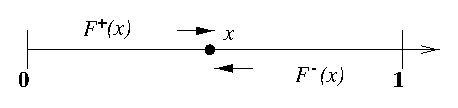
\includegraphics[clip]{1993math-1.eps}}
  \end{center}}

  \begin{subsubquestions}
  \SubSubQuestion
    流量$F^+(x)$と$F^-(x)$を支配する$x$についての一階連立微分方程式
    を導け。

  \SubSubQuestion
    次の行列の固有値および固有ベクトルを求めよ。ただし、固有ベクトルの
    第一成分は1、また、$\alpha>\beta>0$とする。
%
    \[ A = \begin{pmatrix}%
              -\alpha & +\beta \\
              -\beta  & +\alpha \end{pmatrix} \]
%
  \SubSubQuestion
    (ii)の結果を利用して(i)の方程式系を解け。
    ただし、境界条件として粒子は$x=0$で区間に流量1個/秒で流入
    しており、また、$x=1$で区間に流入する粒子は無いとする。さらに
    $a,b>0$とする。
  \end{subsubquestions}


\SubQuestion
  正の整数$N$の分割数$P(N)$、すなわち$N$を$N$以下の正の整数の和で表す
  場合の数を考える。例えば、$N=3$のとき、$N=3=2+1=1+1+1$であるから、
  $P(3)=3$である。また、$P(0)=1$と約束する。このとき次の設問に答えよ。

  \begin{subsubquestions}
  \SubSubQuestion
    $P(4),P(5)$を求めよ。

  \SubSubQuestion
    負でない整数$n$を正の整数$m$以下の正の整数の和で表す場合の数を
    $p(n,m)$と書く。ただし$p(0,m)=1$と約束する。この時分割に現れる
    最大数に着目して$p(n,m)$を$p(n',m'),\\ n'<n,m'\leq m$を用いて
    表しなさい。

  \SubSubQuestion
    (ii)の結果を用いて$P(8)$を求めよ。

  \SubSubQuestion
    問題とする場合の数$q(n)$を係数とする、べき級数
    $h(x)=\ds{\sum_{n=0}^{\infty}q(n)x^n}$を$q(n)$
    の母関数という。例えば、$p(n,2)$に対する母関数は
%
    \[\sum_{n=0}^{\infty}p(n,2)x^n=(1+x^1+x^{1+1}+\cdots)(1+x^2+x^{2+2}+\cdots)\]
%
    で与えられる。これを参考にして$P(N)$の母関数
    $g(x)=\ds{\sum_{n=0}^{\infty}P(n)x^n}$を
    $g(x)=\ds{\prod_{k=0}^{\infty}\frac{1}{f_k(x)}}$の
    形で与える多項式$f_k(k)$を求めよ。
  \end{subsubquestions}
\end{subquestions}
\end{question}
\begin{answer}{教育 数学}{}
\begin{subanswers}
\SubAnswer
  \begin{subsubanswers}
  \SubSubAnswer
    この関数 $f$には特異点はなく、また $r\to\infty$で $f\to 0$
    に収束する。$f$は有限の領域(${\bf R}^2$)に正負の値を持つので
    $f$は${\bf R^2}$上に最大値、最小値を持つ。

    さて、${\bf R^2}$は開集合なので、連続微分可能な関数 $f$がある点で
    最大値または最小値をとるためには、その点で、
%
    \[ \Partial{f}{x} = \Partial{f}{y} = 0 \]
%
    となることが必要条件である。具体的に書き下すと、
%
    \begin{eqnarray}
      +x \bigl[ x^2 - (x^4-y^2)(x^2+y^2) \bigr] &=& 0 \eqname{1-1}\\
      -y \bigl[  1 + 2(x^4-y^2)(x^2+y^2) \bigr] &=& 0 \eqname{1-2}
    \end{eqnarray}
%
    となる。

    $f$が最大値を取るのは明らかに $f$が正の時であり、その時には
    $(x^4-y^2)>0$ なので式\eqhref{1-2}が満たされるためには
    $y=0$となることがわかる。これを式\eqhref{1-1}に代入すると、
%
    \[ 4x^3(1-x^4)=0 \hspace{10mm}%
       \Yueni x=+1,0,-1 \]
%
    が得られる。この時の$f$の値は
%
    \[ f(1,0) = f(-1,0) = \frac{1}{e} \quad f(0,0)=0 \]
%
    なので、最大値は、
%
    \[ f(1,0) = f(-1,0) = \frac{1}{e} \]
%
    である。

    同様にして最小値を求めると、最小値は明らかに負なので
    $(x^4-y^2)<0$ なので式\eqhref{1-1}が満たされるためには
    $x=0$となることがわかる。これを式\eqhref{1-2}に代入すると、
%
    \[ 2y(2y^4-1)=0 \hspace{10mm}%
       \Yueni y=0,\pm \frac{1}{\sqrt[4]{2}} \]
%
    が得られる。この時の$f$の値は
%
    \[ f\Bigl(0,+\frac{1}{\sqrt[4]{2}}\Bigr) =%
       f\Bigl(0,-\frac{1}{\sqrt[4]{2}}\Bigr) =%
      -\frac{1}{\sqrt{2}}e^{-\frac{1}{2}} \qquad f(0,0)=0 \]
%
    なので、最小値は、
%
    \[ f\Bigl(0,+\frac{1}{\sqrt[4]{2}}\Bigr) =%
       f\Bigl(0,-\frac{1}{\sqrt[4]{2}}\Bigr) =%
      -\frac{1}{\sqrt{2}}e^{-\frac{1}{2}} \]
%
    である。

  \SubSubAnswer
    与式を極座標の積分に直すと、
%
    \[ I=\int_{0}^{\infty}\!\!\!\int_{0}^{2\pi}%
         \left( r^5\cos^4\theta-r^3\sin^2\theta \right)%
         e^{-r^4} \d{r}\d{\theta} \]
%
    となる。$\theta$による積分は、
%
    \begin{eqnarray*}
      \int_{0}^{2\pi}\cos^4{\theta}\d{\theta} &=& \int_{0}^{2\pi}
        \left(\frac{1}{4}+\frac{1}{2}\cos2\theta+\frac{1}{8}+
        \frac{1}{8}\cos4\theta\right)\d{\theta}=\frac{3\pi}{4} \\
      \int_{0}^{2\pi}\sin^2{\theta}\d{\theta} &=& \int_{0}^{2\pi}
        \left(\frac{1-\cos2\theta}{2}\right)\d{\theta}=\pi
    \end{eqnarray*}
%
    となる。$r$の積分は、$r^2=t$と変数変換して
%
    \[ I = \pi\int_{0}^{\infty}%
             \left(\frac{3}{8}t^2-\frac{1}{2}t\right)e^{-t^2}\d{t}%
         = \frac{3\pi^{\frac{3}{2}}}{32}-\frac{\pi}{4} \]
%
    と求まる。

  \end{subsubanswers}


\SubAnswer
  \begin{subsubanswers}
  \SubSubAnswer
    正の方向に進む粒子は、$\d{x}$進む間に、$(a+b)F^+\d{x}$個が
    散乱によって失われ、$bF^-\d{x}$個が、負方向に進む粒子からの
    散乱によって生じる。負方向に進む粒子は$-\d{x}$進む間に同様の
    収支があるので結局
%
    \begin{eqnarray*}
      +\Deriver{F^+}{x} &=& -(a+b)F^+ + bF^- \\
      -\Deriver{F^-}{x} &=& -(a+b)F^- + bF^+
    \end{eqnarray*}
%
    となる。

  \SubSubAnswer
    固有値 $\lambda$ は
%
    \[(-\alpha-\lambda)(\alpha-\lambda)+\beta^2=\lambda^2-\alpha^2+\beta^2=0 \hspace{15mm} \Yueni \lambda^{\pm}=\pm\sqrt{\alpha^2-\beta^2} \]
%
    となる。それぞれに対応する固有ベクトルの第2成分を$\gamma^{\pm}$
    とすれば、
%
    \[ \begin{pmatrix}%
         -\alpha & +\beta \\
         -\beta  & +\alpha
       \end{pmatrix}%
       \begin{pmatrix}%
          1 \\ \gamma^{\pm}
       \end{pmatrix}%
       = \pm\sqrt{\alpha^2-\beta^2}%
       \begin{pmatrix}%
          1 \\ \gamma^{\pm}
       \end{pmatrix} \]
%
    となるので、
%
    \[ \gamma^{\pm}=\frac{\alpha\pm\sqrt{\alpha^2-\beta^2}}{\beta} \]
%
    が得られる。よって固有ベクトルは、
%
    \[ \begin{pmatrix}%
         1 \\ (\alpha+\sqrt{\alpha^2-\beta^2})/\beta
       \end{pmatrix}%
       ,\hspace{10mm}%
       \begin{pmatrix}%
         1 \\ (\alpha-\sqrt{\alpha^2-\beta^2})/\beta
       \end{pmatrix} \]
%
    となる。ただし、複号の順序は、固有値と固有ベクトルのそれぞれで
    一致している。

  \SubSubAnswer
    $\alpha=a+b,\beta=b$とすれば、(i)の方程式は、
%
    \[ \Deriver{}{x} \begin{pmatrix}%
         F^+ \\ F^-
       \end{pmatrix}
       =%
       \begin{pmatrix}%
         -\alpha & +\beta  \\ 
         -\beta  & +\alpha
       \end{pmatrix}%
       \begin{pmatrix}%
         F^+ \\ F^-
       \end{pmatrix} \]
%
    となる。この行列を対角化するために、
%
    \[ \begin{pmatrix}%
         F^+ \\ F^-
       \end{pmatrix}%
       =%
       \begin{pmatrix}%
         1          & 1          \\
         \gamma^{+} & \gamma^{-}
       \end{pmatrix}%
       \begin{pmatrix}%
         F^{+\prime} \\ F^{-\prime}
       \end{pmatrix}%
    \]
%
    で変換すると
%
    \[ \Deriver{}{x} \begin{pmatrix}%
         F^{+\prime} \\ F^{-\prime}
       \end{pmatrix}%
       =%
       \begin{pmatrix}%
         \lambda^+ & 0 \\
         0 & \lambda^-
       \end{pmatrix}%
       \begin{pmatrix}%
         F^{+\prime} \\ F^{-\prime}
       \end{pmatrix} \]
%
    となる。よってこの解は
%
    \[ F^{+\prime}(x) = A^+ e^{\lambda^+ x} \hspace{10mm}%
       F^{-\prime}(x) = A^- e^{\lambda^- x} \]
%
    であり、変換して
%
    \begin{eqnarray*}
      F^+(x) &=& A^+ e^{\lambda^+x} + A^- e^{\lambda^-x} \\
      F^-(x) &=& A^+\gamma^+e^{\lambda^+x}+A^-\gamma^-e^{\lambda^-x}
    \end{eqnarray*}
%
    となる。境界条件 $F^+(0)=1,F^-(1)=0$を用いて未定係数 $A^+,A^-$
    を定めて、さらに $\lambda^-=-\lambda^+\equiv \lambda$、
    $\gamma^+\gamma^-=1$の関係を用いると、結局
%
    \begin{eqnarray*}
      F^+(x) &=& \frac{%
                   \gamma^-e^{\lambda^-+\lambda^+x}%
                  -\gamma^+e^{\lambda^++\lambda^-x}%
                 }{
                   \gamma^-e^{\lambda^-}%
                  -\gamma^+e^{\lambda^+}%
                 } 
              =  \frac{%
                   \gamma^-e^{-\lambda(1-x)}%
                  -\gamma^+e^{+\lambda(1-x)}%
                 }{
                   \gamma^-e^{-\lambda}%
                  -\gamma^+e^{+\lambda}%
                 } \\
      F^-(x) &=& \frac{%
                   \gamma^+\gamma^-e^{\lambda^-+\lambda^+x}%
                  -\gamma^+\gamma^-e^{\lambda^++\lambda^-x}%
                 }{
                   \gamma^-e^{\lambda^-}%
                  -\gamma^+e^{\lambda^+}%
                 }
              =  \frac{%
                   e^{-\lambda(1-x)}%
                  -e^{+\lambda(1-x)}%
                 }{
                   \gamma^-e^{-\lambda}%
                  -\gamma^+e^{+\lambda}%
                 }
    \end{eqnarray*}
%
    となる。

  \end{subsubanswers}


\newpage
\SubAnswer
  \begin{subsubanswers}
  \SubSubAnswer
    $4=1+1+1+1=2+1+1=3+1=2+2$だから、$P(4)=5$ \\
    $5=1+1+1+1+1=2+1+1+1=3+1+1=4+1=2+2+1=3+2$だから、$P(5)=7$

  \SubSubAnswer
    $p(n,m)$は$m$以下の数で$n$を分割する種類の数であるが、
    分割した項の中で一番大きい数が$k$であるような分割の種類の数は、
    残りの和が $n-k$ で$k$以下の数で分割する分割の種類の数 $p(n-k.k)$
    であるので、よって
%
    \[ p(n,m) = \sum_{k=1}^{m} p(n-k.k) \]
%
    と表されることになる。


  \SubSubAnswer
    (ii)で得られた公式を使って順に計算していく。
%
    \begin{eqnarray*}
      p(8)&=&p(8,8) \\
          &=&p(7,1)+p(6,2)+p(5,3)+p(4,4)+p(3,5)+p(2,6)+p(1,7)+p(0,8)\\
          &=&1+\{p(5,1)+p(4,2)\}+\{p(4,1)+p(3,2)+p(2,3)\}+5+3+2+1+1\\
          &=&1+(1+3)+(1+2+2)+5+3+2+1+1\\
          &=&22
    \end{eqnarray*}

  \SubSubAnswer
    与えられている $p(n,2)$ の母関数の右辺の表式を展開して、
    $x$ の各次数ごとを眺めると
%
    \begin{eqnarray*}
      x^0 &:& 1 \\
      x^1 &:& x^{1} \\
      x^2 &:& x^{2} + x^{1+1} \\
      x^3 &:& x^{2+1} + x^{1+1+1}
    \end{eqnarray*}
%
    のように$x$の指数は分割の仕方を示していることがわかる。

    これをヒントに整数$n$の一般の分割を考える。\\
%
    整数$n$の和分割で、整数 $m\,(m=[1,\infty))$の数の項の数を $a_m$ と
    と表すことにする。この分割を$x$の指数で示すと
%
    \[ x^n = x^{1a_1+2a_2+3a_3+\cdots}%
           = x^{1a_1}x^{2a_2}x^{3a_3} \cdots \]
%
    となる。これを逆に考えると、任意の数の組 $\{a_m\}\,(m=[1,\infty))$
    は、上式で計算される $n$の分割の一例になっている。\\
%
    ここで$p(n,2)$の例を思い出して
%
    \[ (1+x+x^2+\cdots)(1+x^2+x^4+\cdots)(1+x^3+x^6+\cdots)\cdots\]
%
    という式を考える。これを展開すると $x$の$n$次の項の係数は
    $n$の分割の種類の数となっている。すなわち、これは$P(n)$の母関数
    である。
%
    \begin{eqnarray*}
      \sum_{n=0}^{\infty} P(n)x^n%
       &=&(1+x+x^2+\cdots)(1+x^2+x^4+\cdots)(1+x^3+x^6+\cdots)\cdots\\
       &=&\frac{1}{1-x}\frac{1}{1-x^2}\frac{1}{1-x^3}\cdots%
       = \prod_{k=1}^{\infty}\frac{1}{1-x^k} = \prod_{k=0}^{\infty}\frac{1}{1-x^{k+1}}
    \end{eqnarray*}
%
    となる。よって
%
    \[ f_k(x) = 1-x^{k+1} \]
%
    と求まる。

  \end{subsubanswers}

\end{subanswers}
\end{answer}


\end{document}
